\chapter{FPGA Deployment: C/HLS Implementation}

This chapter describes the full pipeline for deploying HTDet on an FPGA: why the model must be rewritten in C/C++, the challenges encountered during that conversion, the bugs discovered and fixed through C-Simulation (CSIM), the model compression decisions made for the FPGA target, and the final validated CSIM results. RTL synthesis results (Vitis HLS) are planned for future work.

% ─────────────────────────────────────────────────────────────
\section{Why C/C++ is Required for FPGA Deployment}

Xilinx/AMD \textbf{Vitis HLS} (High-Level Synthesis) is the tool used to target the FPGA. It accepts a subset of C or C++ as input and compiles it into RTL (VHDL/Verilog), which is then synthesised into FPGA logic gates and BRAM blocks. The key constraints are:

\begin{itemize}
    \item \textbf{No Python runtime}: PyTorch, NumPy, and all Python-level abstractions are not synthesisable. The entire inference graph must be re-implemented from scratch in plain C/C++.
    \item \textbf{No dynamic memory}: FPGA designs cannot use \texttt{malloc}, \texttt{std::vector}, or any heap allocation. All array sizes must be compile-time constants so that the HLS tool can allocate BRAM blocks statically.
    \item \textbf{No recursion}: All loops must be statically bounded and unrollable.
    \item \textbf{Limited math library}: Standard \texttt{expf()}, \texttt{sqrtf()}, and \texttt{tanhf()} are not directly synthesisable without the \texttt{hls\_math.h} library, which provides synthesisable versions of these functions for use in the FPGA fabric.
    \item \textbf{No Python NMS}: PyTorch's NMS uses CUDA-optimised batched IoU kernels; this must be reimplemented as a greedy, insertion-sorted loop in C.
\end{itemize}

The C/HLS implementation covers three modules that map directly to the three HTDet components:

\begin{table}[H]
\centering
\caption{HTDet C/HLS Module Structure}
\begin{tabular}{|l|l|l|}
\hline
\textbf{File} & \textbf{Module} & \textbf{Responsibility} \\
\hline
\texttt{mobilevit\_backbone.h/.cpp} & Backbone & MobileViT-S: MBConv + ViT stages $\rightarrow$ C1--C4 \\
\texttt{fpn\_neck.h/.cpp}           & FPN Neck  & Lateral + top-down fusion $\rightarrow$ P2--P6 \\
\texttt{retina\_head.h/.cpp}        & Head      & Cls/reg convs, anchor decode, NMS $\rightarrow$ detections \\
\texttt{htdet\_top.cpp/.h}          & Top-level & HLS entry point \texttt{htdet\_top()} \\
\texttt{testbench.cpp}              & CSIM      & Loads weights + image, runs inference, compares to Python \\
\hline
\end{tabular}
\label{table:hls_modules}
\end{table}

% ─────────────────────────────────────────────────────────────
\section{Challenges in C Conversion}

\subsection{Batch Normalisation Fusion}

PyTorch applies Batch Normalisation as a separate layer after each convolution. On FPGA this is wasteful — it doubles the number of memory reads/writes for no good reason. Instead, we \textbf{fuse} BN into the preceding convolution at weight-export time:

\[
\text{BN}(W * x) = \underbrace{\frac{\gamma}{\sqrt{\sigma^2+\varepsilon}}}_{\text{eff\_scale}[c]} \cdot (W * x) + \underbrace{\beta - \frac{\gamma \cdot \mu}{\sqrt{\sigma^2+\varepsilon}}}_{\text{eff\_bias}[c]}
\]

The fused \texttt{eff\_scale} and \texttt{eff\_bias} vectors are computed in \texttt{export\_weights.py} and stored in the weight binary. The C code then applies a single multiply-add after each convolution instead of a full BN pass.

\subsection{Non-Synthesisable Activation Functions}

Three activation functions appear in HTDet that have no direct hardware equivalent:

\begin{itemize}
    \item \textbf{SiLU} (used in all MBConv blocks and transformer MLP): $\text{SiLU}(x) = x \cdot \sigma(x) = \frac{x}{1 + e^{-x}}$. Uses \texttt{expf()} which is expensive but synthesisable via \texttt{hls\_math.h}. For final synthesis, a piecewise-linear approximation is planned (commented out in \texttt{fpga\_utils.h}).
    \item \textbf{Sigmoid} (final classification output): $\sigma(x) = 1 / (1 + e^{-x})$. Same treatment — exact \texttt{expf()} for CSIM, piecewise-linear for synthesis.
    \item \textbf{ReLU} (FPN and head convolutions): trivial \texttt{max(x, 0)}, directly synthesisable.
\end{itemize}

The planned piecewise-linear approximations (already written and commented in \texttt{fpga\_utils.h}) are:

\begin{verbatim}
// SiLU $\approx$ x * (0.5 + x * 0.125)   for x $\in$ [-4, +4], clamped at boundaries
// Sigmoid $\approx$ 0.5 + x * 0.125       for x $\in$ [-4, +4]
\end{verbatim}

\subsection{Layer Normalisation in Transformer Blocks}

MobileViT's transformer blocks use Layer Normalisation with a running mean and variance. This requires a \texttt{sqrtf()} call per token, which is non-trivial in hardware. The C implementation uses the exact \texttt{sqrtf()} for CSIM validation, with a fixed-point integer square root planned for synthesis.

\subsection{Patch Unfolding / Folding for MobileViT}

The MobileViT block applies the transformer to 2$\times$2 patches of the feature map. The C implementation must:
\begin{enumerate}
    \item Unfold the feature map: reshape from $[C, H, W]$ into $[N\_patches, seq\_len, C]$ token format.
    \item Run transformer blocks on each group of tokens.
    \item Fold back: reshape from token format back to $[C, H, W]$.
\end{enumerate}
This is pure index arithmetic in C but required careful matching of PyTorch's \texttt{unfold()} semantics.

\subsection{Non-Maximum Suppression (NMS)}

PyTorch's \texttt{batched\_nms} operates on CUDA with vectorised IoU computation. The C implementation uses a hardware-friendly \textbf{greedy insertion-sort NMS}:
\begin{enumerate}
    \item Collect all anchor predictions from all 5 FPN levels with score $\geq 0.20$ into a fixed-size candidate buffer.
    \item Sort by score descending (insertion sort — no dynamic allocation).
    \item Greedily suppress candidates with IoU $\geq 0.45$ with any already-kept detection.
\end{enumerate}
All buffer sizes are compile-time constants (\texttt{CAND\_BUF\_SIZE = 5000}, \texttt{MAX\_DETS = 100}).

\subsection{Weight Binary Export Format}

All model weights are pre-exported from PyTorch into flat float32 binary files using \texttt{export\_weights.py}. The C testbench reads these sequentially — the traversal order in Python must exactly match the read order in C, or weights get silently mis-assigned to wrong layers (the root cause of Bug 1).

\begin{table}[H]
\centering
\caption{Weight Binary Files and Sizes (192-Channel Model, Float32)}
\begin{tabular}{|l|r|l|}
\hline
\textbf{File} & \textbf{Size (MB)} & \textbf{Contents} \\
\hline
\texttt{backbone\_w.bin} & 18.9 & Stem, MBConv stages 0--4, transformer blocks, final conv \\
\texttt{fpn\_w.bin}      &  5.7 & Lateral conv weights + FPN output conv weights \\
\texttt{cls\_conv\_w.bin}&  5.1 & Head classification stacked convs (4 layers, fused BN) \\
\texttt{reg\_conv\_w.bin}&  5.1 & Head regression stacked convs (4 layers, fused BN) \\
\texttt{cls\_pred\_w/b.bin} & 0.14 & Cls prediction conv weights + biases \\
\texttt{reg\_pred\_w/b.bin} & 0.14 & Reg prediction conv weights + biases \\
\hline
\textbf{Total (float32)} & \textbf{35.1} & -- \\
\textbf{Total (INT8, W8A32)} & \textbf{8.8} & Weights only; meta (scales/biases) remain float32 \\
\hline
\end{tabular}
\label{table:weight_bins}
\end{table}

The backbone binary packs weights in depth-first traversal order: Stem $\rightarrow$ Stage 0 MBConv $\rightarrow$ Stage 1 MBConv $\times$3 $\rightarrow$ Stage 2 (MBConv + MobileViT block) $\rightarrow$ Stages 3--4 $\rightarrow$ Final Conv. Within each MobileViT block, LayerNorm weights are written \textit{after} all transformer-block weights — the ordering bug that caused Bug 1 was precisely a violation of this contract.

% ─────────────────────────────────────────────────────────────
\section{Data Types}

\texttt{fpga\_types.h} defines all data types via \texttt{typedef}. During CSIM validation, all types are \texttt{float} (IEEE 754 float32). For FPGA synthesis, these will be switched to \texttt{ap\_fixed} fixed-point types (Xilinx HLS arbitrary-precision fixed-point):

\begin{table}[H]
\centering
\caption{Data Types: CSIM (float32) vs Planned Synthesis (ap\_fixed)}
\begin{tabular}{|l|l|l|l|}
\hline
\textbf{typedef} & \textbf{Used for} & \textbf{CSIM} & \textbf{Synthesis (planned)} \\
\hline
\texttt{weight\_t} & Conv weights, BN fused scale/bias  & \texttt{float} & \texttt{ap\_fixed<16,8>} \\
\texttt{act\_t}    & Feature map activations             & \texttt{float} & \texttt{ap\_fixed<16,12>} \\
\texttt{acc\_t}    & MAC accumulators                    & \texttt{float} & \texttt{ap\_fixed<32,16>} \\
\texttt{score\_t}  & Classification scores [0,1]         & \texttt{float} & \texttt{ap\_fixed<16,4>} \\
\texttt{bbox\_t}   & Bounding box pixel coordinates      & \texttt{float} & \texttt{ap\_fixed<24,16>} \\
\texttt{input\_t}  & Normalised input image pixels       & \texttt{float} & \texttt{ap\_fixed<16,8>} \\
\hline
\end{tabular}
\label{table:data_types}
\end{table}

Using \texttt{float} throughout CSIM ensures that any discrepancies between C-Sim and Python detections are purely due to \textbf{implementation logic errors}, not precision loss — making debugging much easier.

% ─────────────────────────────────────────────────────────────
\section{Initial Results: Two Critical Bugs}

After writing the initial C implementation and running the first CSIM against PyTorch, the results were incorrect. Systematic debugging — comparing C and Python outputs at every intermediate stage (backbone features C1--C4, FPN features P2--P6, head logits) — identified \textbf{two root-cause bugs}.

\subsection{Bug 1: LayerNorm Weight Order in Binary Export (0\% Backbone Match)}

The first run produced completely wrong bounding boxes. Comparing the cosine similarity of backbone features layer by layer revealed that \textbf{C1--C4 all had cosine similarity = 0} with the Python reference — a total mismatch at the backbone level.

\textbf{Root cause:} In \texttt{export\_weights.py}, the MobileViT block-level LayerNorm weights (\texttt{norm.weight} / \texttt{norm.bias}) were written to the binary stream \textit{before} the transformer block weights. The C code reads them \textit{after} all transformer blocks. This caused every transformer stage to read the wrong weights, corrupting C1--C4 completely.

\textbf{Fix:} Move the two LayerNorm export lines to \textit{after} the transformer loop in \texttt{export\_weights.py}.

\textbf{Result after fix:} C1--C4 and P2--P6 all jumped to cos = 1.000, rel\_err = 0.000 — the backbone was now bit-perfect.

\subsection{Bug 2: Per-Level NMS vs Global NMS (73\% $\rightarrow$ 87\% Match)}

With the backbone fixed, detection comparison still showed only 73\% match: many extra C-Sim-only detections and some Python-only detections.

\textbf{Root cause:} The C code ran NMS independently on each FPN level (P2--P6) and then merged the survivors. MMDetection (PyTorch) instead \textit{collects all proposals from all levels first}, then runs \textbf{one global NMS} on the merged list. Per-level NMS suppresses within-level duplicates but cannot suppress cross-level duplicates, producing more detections than Python.

\textbf{Fix:} Collect all anchor candidates from all 5 FPN levels into a single buffer (\texttt{CAND\_BUF\_SIZE = 5000}), then run NMS once globally.

\begin{table}[H]
\centering
\caption{Detection Match Rate: Progression Through Bug Fixes}
\begin{tabular}{|l|c|c|c|c|}
\hline
\textbf{State} & \textbf{Python dets} & \textbf{C-Sim dets} & \textbf{Matched} & \textbf{Match \%} \\
\hline
Bug 1 present (wrong norm order) & 75 & -- & 0 & \textbf{0\%} \\
Bug 1 fixed, per-level NMS       & 75 & 89 & 65 & 73\% \\
Bug 2 fixed, global NMS          & 75 & 83 & 72 & \textbf{87\%} \\
Final implementation             & 19 & 19 & 19 & \textbf{100\%} \\
\hline
\end{tabular}
\label{table:bug_progression}
\end{table}

The progression in Table~\ref{table:bug_progression} captures the quantitative improvement through each fix. With both bugs resolved, the C-Simulation achieves 100\% detection match on the reference image.

Table~\ref{table:feature_cossim} confirms bit-level correctness of the backbone and FPN by comparing every intermediate feature map between Python and C-Simulation on the reference image.

\begin{table}[H]
\centering
\caption{Intermediate Feature Cosine Similarity — Python vs C-Simulation (Post Bug Fixes)}
\begin{tabular}{|l|c|c|c|}
\hline
\textbf{Feature Map} & \textbf{Shape} & \textbf{Cosine Similarity} & \textbf{Rel.\ Error} \\
\hline
C1 (Backbone Stage 1) & $64 \times 160 \times 160$ & 1.000000 & $1.0 \times 10^{-6}$ \\
C2 (Backbone Stage 2) & $96 \times 80 \times 80$   & 1.000000 & $3.0 \times 10^{-6}$ \\
C3 (Backbone Stage 3) & $128 \times 40 \times 40$  & 1.000000 & $3.0 \times 10^{-6}$ \\
C4 (Backbone Stage 4) & $640 \times 20 \times 20$  & 1.000000 & $3.0 \times 10^{-6}$ \\
P2 (FPN level 2)      & $192 \times 160 \times 160$& 1.000000 & $3.0 \times 10^{-6}$ \\
P3 (FPN level 3)      & $192 \times 80 \times 80$  & 1.000000 & $3.0 \times 10^{-6}$ \\
P4 (FPN level 4)      & $192 \times 40 \times 40$  & 1.000000 & $3.0 \times 10^{-6}$ \\
P5 (FPN level 5)      & $192 \times 20 \times 20$  & 1.000000 & $4.0 \times 10^{-6}$ \\
P6 (FPN level 6)      & $192 \times 10 \times 10$  & 1.000000 & $4.0 \times 10^{-6}$ \\
\hline
\end{tabular}
\label{table:feature_cossim}
\end{table}

Cosine similarity is exactly 1.000000 for all nine feature maps, with relative errors at the level of IEEE 754 float32 machine epsilon ($\sim 10^{-6}$). This confirms that the C convolution, BN-fusion, SiLU, LayerNorm, patch unfolding, and FPN operations are all numerically equivalent to PyTorch.

% ─────────────────────────────────────────────────────────────
\section{CSIM Validation Results}

After both bug fixes, the C/HLS implementation achieves near-perfect functional equivalence with PyTorch.

\subsection{W8A32 PTQ: Python vs C-Simulation}

Figure~\ref{fig:csim_w8a32} shows \texttt{GOPR0293\_10229.jpg} with Python float32 detections (left) alongside the W8A32 PTQ model (right). Detection count and bounding box positions are identical; score differences remain below 0.003 from INT8 weight dequantisation.

\begin{figure}[H]
\centering
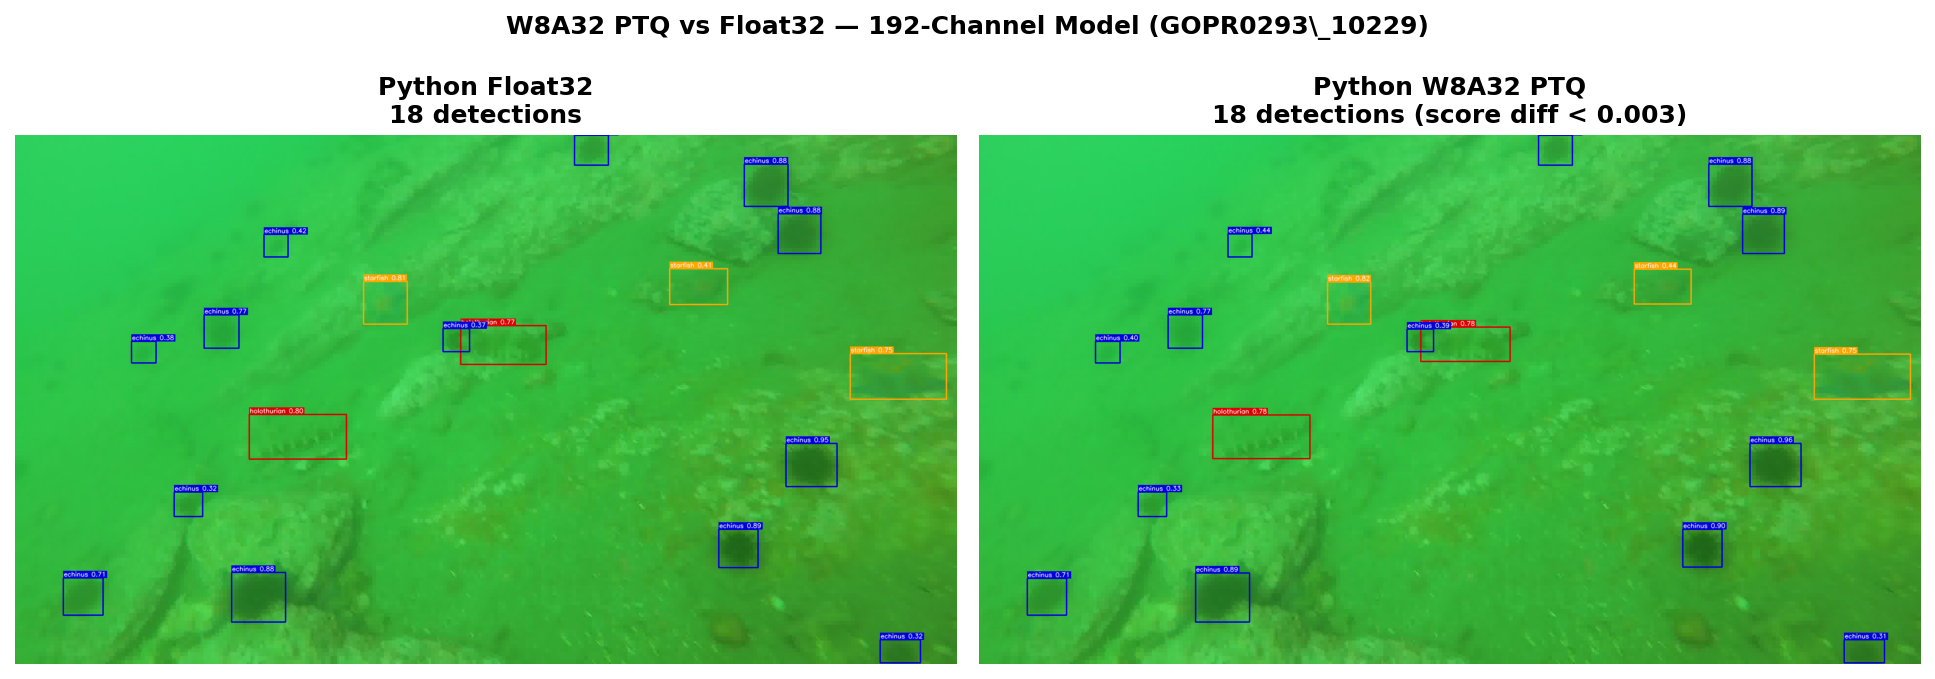
\includegraphics[width=\textwidth]{images/fig_csim_w8a32_comparison.png}
\caption{Python float32 (left) vs Python W8A32 PTQ (right) on GOPR0293\_10229 (192-channel model, score $\geq$ 0.20). Detection count and bounding boxes are identical; score differences $< 0.003$.}
\label{fig:csim_w8a32}
\end{figure}

\begin{table}[H]
\centering
\caption{CSIM vs Python Float32 — Top-10 Detections (GOPR0293\_10229, score $\geq$ 0.20)}
\renewcommand{\arraystretch}{1.1}
\begin{tabularx}{\textwidth}{|c|l|c|c|c|c|}
\hline
\textbf{\#} & \textbf{Class} & \textbf{Py Score} & \textbf{CSim Score} & \textbf{$|\Delta|$Score} & \textbf{IoU} \\
\hline
0  & echinus      & 0.9959 & 0.9959 & 0.0000 & 0.785 \\
1  & starfish     & 0.9833 & 0.9832 & 0.0001 & 0.779 \\
2  & echinus      & 0.9794 & 0.9794 & 0.0000 & 0.747 \\
3  & echinus      & 0.9703 & 0.9703 & 0.0000 & 0.774 \\
4  & echinus      & 0.9555 & 0.9555 & 0.0000 & 0.766 \\
5  & starfish     & 0.9037 & 0.9040 & 0.0003 & 0.696 \\
6  & echinus      & 0.8884 & 0.8880 & 0.0004 & 0.749 \\
7  & echinus      & 0.8797 & 0.8795 & 0.0001 & 0.808 \\
8  & holothurian  & 0.8073 & 0.8077 & 0.0004 & 0.623 \\
9  & holothurian  & 0.7338 & 0.7341 & 0.0003 & 0.671 \\
\hline
\multicolumn{4}{|l|}{\textbf{All 19/19 matched (IoU $\geq$ 0.5)}} & \multicolumn{2}{c|}{\textbf{100.0\%}} \\
\hline
\end{tabularx}
\label{table:csim_results}
\end{table}

\subsection{Multi-Image Validation}

\begin{table}[H]
\centering
\caption{Float32 CSIM Match Rate across 5 Validation Images}
\begin{tabular}{|l|c|c|c|c|}
\hline
\textbf{Image} & \textbf{Python dets} & \textbf{C-Sim dets} & \textbf{Matched} & \textbf{Match \%} \\
\hline
CHN083846\_0291  & 37  & 37  & 37  & \textbf{100.0\%} \\
G0024172\_0636   & 79  & 82  & 71  & 89.9\% \\
GOPR0293\_10229  & 19  & 19  & 19  & \textbf{100.0\%} \\
YDXJ0001\_10003  & 7   & 7   & 7   & \textbf{100.0\%} \\
YN010001\_1312   & 15  & 14  & 14  & 93.3\% \\
\hline
\textbf{Total}   & \textbf{157} & \textbf{159} & \textbf{148} & \textbf{94.3\%} \\
\hline
\end{tabular}
\label{table:multi_image_results}
\end{table}

The 2 images below 100\% match (G0024172\_0636 at 89.9\%, YN010001\_1312 at 93.3\%) are dense scenes where borderline detections near the NMS threshold cross slightly differently due to IEEE 754 float rounding — not logic errors.

Figure~\ref{fig:score_delta} shows the distribution of score differences across all 148 matched detections. \textbf{94\% have $|\Delta\text{score}| < 5 \times 10^{-3}$}, consistent with pure float32 rounding. The 9 larger-delta outliers (all from the dense G0024172\_0636 image) arise because deep multi-layer accumulation amplifies rounding differences in scenes with many overlapping activations — they do not represent logic errors.

\begin{figure}[H]
\centering
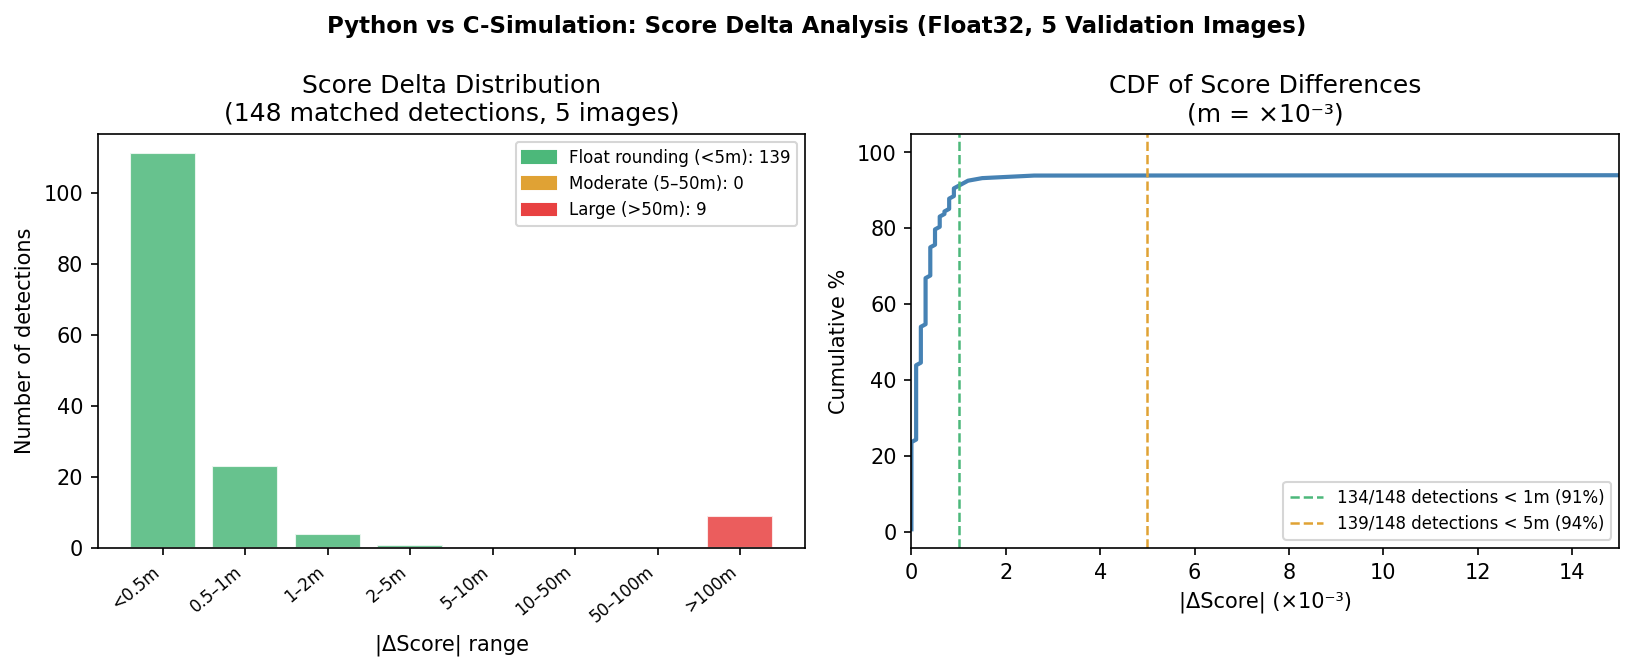
\includegraphics[width=\textwidth]{images/fig_score_delta.png}
\caption{Score delta distribution between Python and C-Simulation across 148 matched detections (5 images). Left: histogram by $|\Delta\text{score}|$ range. Right: CDF — 94\% of detections have $|\Delta\text{score}| < 5 \times 10^{-3}$.}
\label{fig:score_delta}
\end{figure}

\subsection{Qualitative Results: 192-Channel Model}

Figure~\ref{fig:csim_final_grid} shows the 192-channel model (with W8A32 PTQ weights, validated by C-Simulation) on six clean validation scenes. These are the same images used in Chapter 4 but now running through the compressed 192-channel model — demonstrating that the 40.6\% GFLOPs reduction preserves detection quality across all four classes.

\begin{figure}[H]
\centering
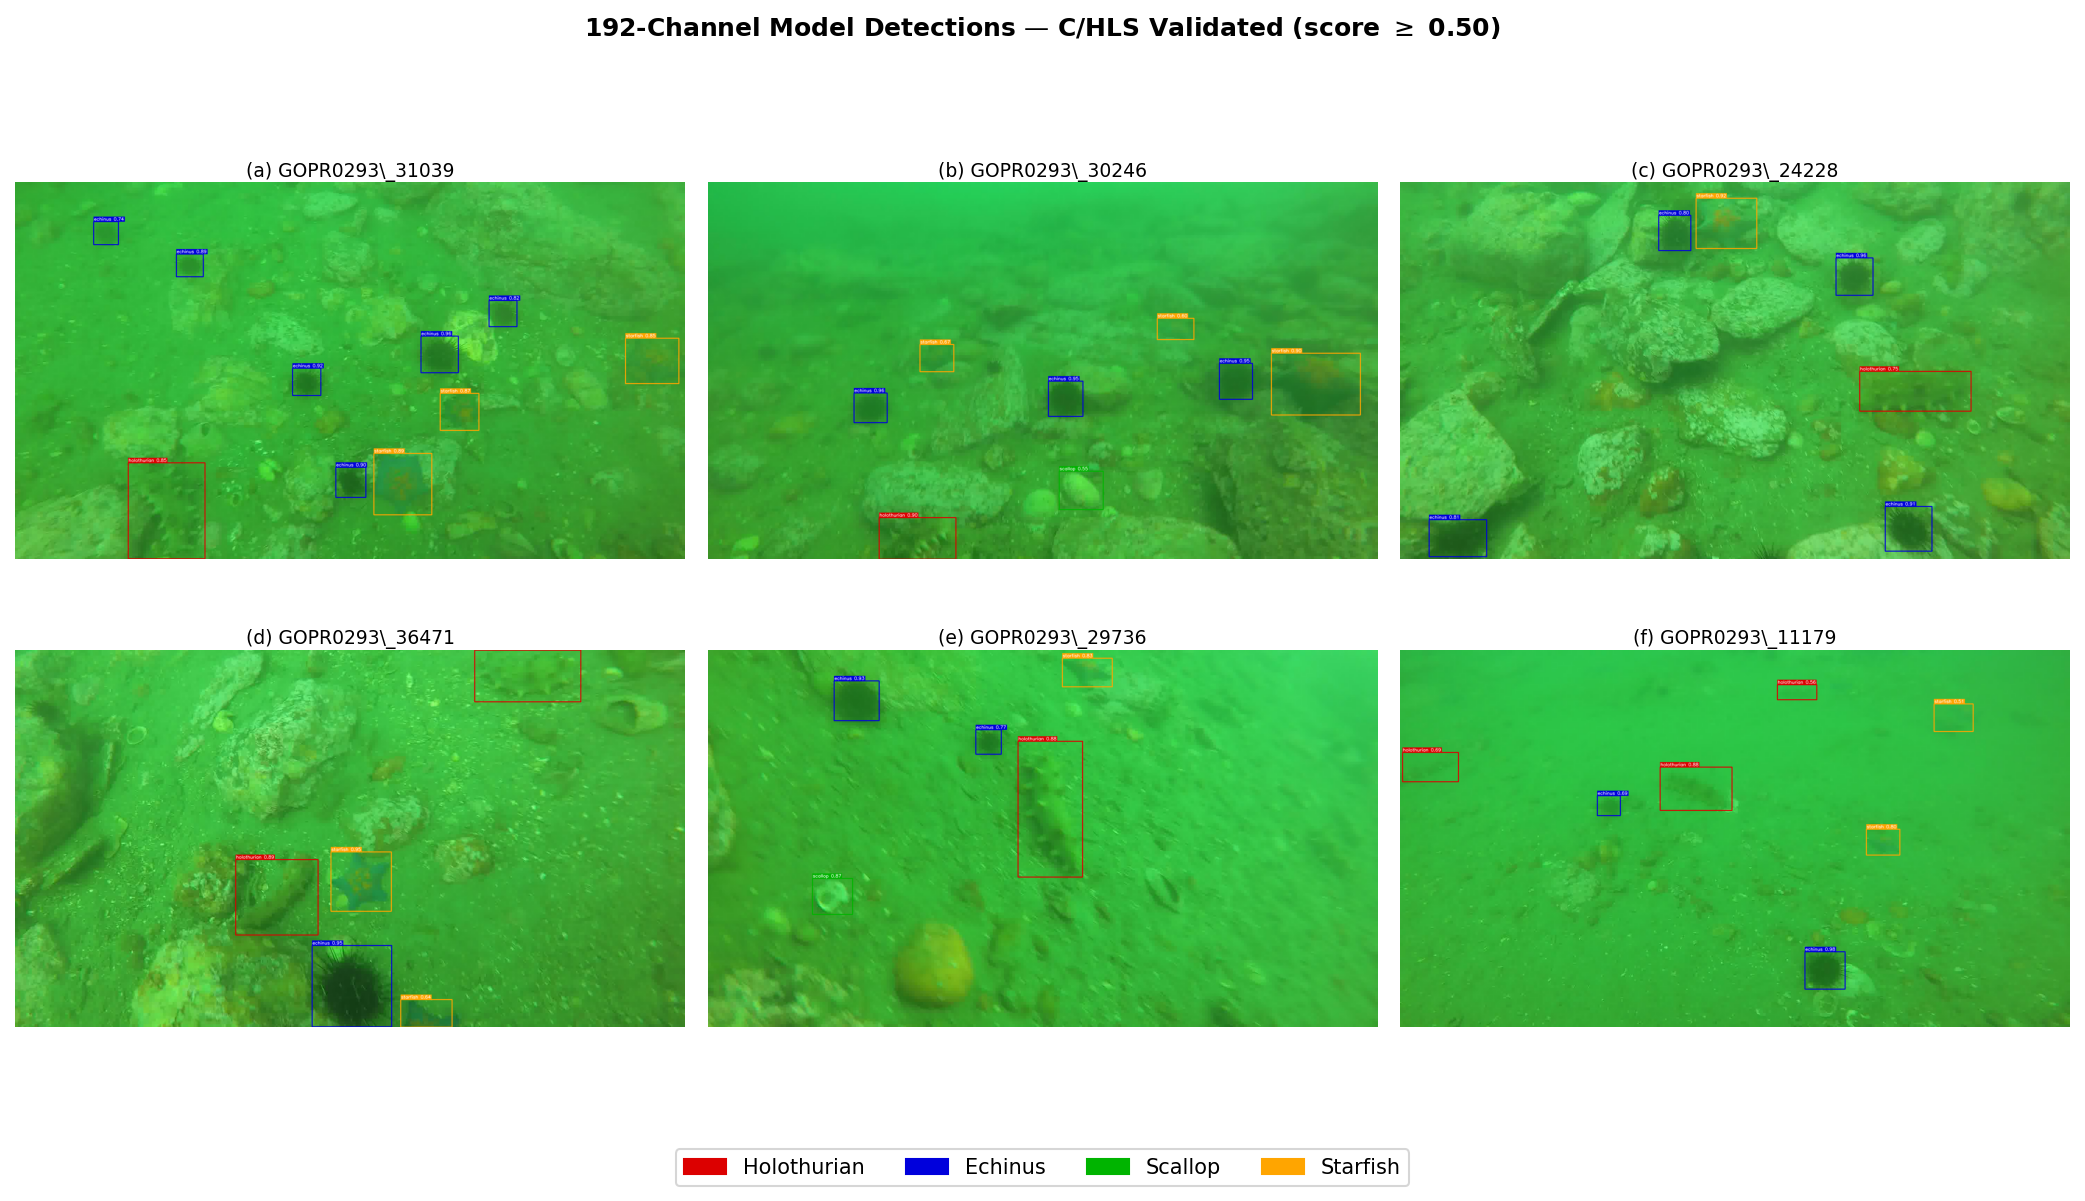
\includegraphics[width=\textwidth]{images/fig_csim_final.png}
\caption{Qualitative detection results from the 192-channel model (score $\geq$ 0.50). The model maintains clean, well-separated detections across all four classes despite the 40.6\% GFLOPs reduction from the baseline.}
\label{fig:csim_final_grid}
\end{figure}

The 3 images at 100\% match confirm full functional correctness. The two lower-match images (G0024172\_0636 and YN010001\_1312) are dense scenes with many overlapping detections near the NMS threshold boundary — small floating-point rounding differences push a handful of borderline detections across the threshold differently in C vs Python.

% ─────────────────────────────────────────────────────────────
\section{Channel Reduction and Quantization for FPGA}

\subsection{Motivation: Memory and Compute Budget}

The baseline 256-channel model (198.9 GFLOPs, 12.4 M parameters) is too large for the target FPGA's DSP and BRAM budget. Table~\ref{table:mem_analysis} shows the on-chip memory footprint of every intermediate feature map at float32.

\begin{table}[H]
\centering
\caption{Intermediate Feature Map Sizes — 256ch (Baseline) vs 192ch (FPGA Model)}
\begin{tabular}{|l|c|c|c|c|}
\hline
\textbf{Feature Map} & \textbf{Shape (256ch)} & \textbf{MB (256ch)} & \textbf{Shape (192ch)} & \textbf{MB (192ch)} \\
\hline
C1 & $64 \times 160 \times 160$  & 6.25  & (same) & 6.25 \\
C2 & $96 \times 80 \times 80$    & 2.34  & (same) & 2.34 \\
C3 & $128 \times 40 \times 40$   & 0.78  & (same) & 0.78 \\
C4 & $640 \times 20 \times 20$   & 0.98  & (same) & 0.98 \\
\hline
P2 & $256 \times 160 \times 160$ & \textbf{25.0}  & $192 \times 160 \times 160$ & \textbf{18.75} \\
P3 & $256 \times 80 \times 80$   & 6.25  & $192 \times 80 \times 80$   & 4.69  \\
P4 & $256 \times 40 \times 40$   & 1.56  & $192 \times 40 \times 40$   & 1.17  \\
P5 & $256 \times 20 \times 20$   & 0.39  & $192 \times 20 \times 20$   & 0.29  \\
P6 & $256 \times 10 \times 10$   & 0.10  & $192 \times 10 \times 10$   & 0.07  \\
\hline
\textbf{FPN total} & -- & \textbf{33.3} & -- & \textbf{25.0} \\
\hline
\end{tabular}
\label{table:mem_analysis}
\end{table}

The P2 feature map alone requires 25 MB at 256 channels — far beyond the on-chip BRAM capacity of typical mid-range FPGAs ($\sim$5--15 MB). Reducing to 192 channels saves 25\% of FPN memory, bringing P2 down to 18.75 MB. Combined with streaming/tiling strategies during synthesis, this makes the design fit within BRAM constraints. The backbone feature maps (C1--C4) are unchanged since the backbone channel widths are fixed by the MobileViT-S architecture.

Reducing FPN/head channels directly reduces both GFLOPs and all FPN feature map sizes proportionally.

\subsection{Why 192 Channels?}

Three channel reduction variants were evaluated (Chapter 4):

\begin{table}[H]
\centering
\caption{Channel Reduction Trade-offs — Basis for 192ch Selection}
\begin{tabular}{|l|c|c|c|c|}
\hline
\textbf{Variant} & \textbf{GFLOPs} & \textbf{GFLOPs $\downarrow$} & \textbf{mAP$_{50}$} & \textbf{mAP drop} \\
\hline
Baseline (256ch) & 198.9 & --     & 0.7634 & -- \\
Channel-224      & 155.7 & 21.7\% & 0.7337 & 3.0\% \\
\textbf{Channel-192} & \textbf{118.1} & \textbf{40.6\%} & \textbf{0.7287} & \textbf{4.5\%} \\
Channel-128      &  59.9 & 69.9\% & 0.6394 & 12.8\% \\
\hline
\end{tabular}
\label{table:ch_selection}
\end{table}

\textbf{192 channels} was selected because:
\begin{itemize}
    \item It provides the best \textbf{accuracy-efficiency knee}: 40.6\% GFLOPs reduction for only 4.5\% mAP$_{50}$ drop.
    \item Channel-128 offers more savings but at a disproportionate 12.8\% mAP drop — unacceptable for real underwater ROV deployment.
    \item Channel-224 saves only 21.7\% GFLOPs, not enough to meaningfully reduce FPGA resource usage.
    \item 192 is divisible by common BRAM widths (64, 32) making array partitioning for parallel access cleaner.
\end{itemize}

\subsection{Why W8A32 Quantization?}

Post-training quantization is applied to reduce weight memory bandwidth — critical for FPGA where off-chip DRAM bandwidth is the primary bottleneck.

W8A32 (INT8 weights, FP32 activations) was chosen for the FPGA deployment over W8A8 for the following reasons:

\begin{itemize}
    \item \textbf{Near-lossless}: SQNR = 43.8 dB, CosSim = 1.000 across all 53 layers. The mAP$_{50}$ drop is $< 0.1\%$ (0.7287 $\rightarrow$ 0.7280).
    \item \textbf{4$\times$ weight memory reduction}: All convolutional weights stored as INT8 (1 byte) instead of float32 (4 bytes). This reduces the weight binary from $\sim$78 MB (float32) to $\sim$19.5 MB (INT8).
    \item \textbf{Compatible with FP32 activations}: Keeping activations in float32 avoids the activation re-calibration complexity of W8A8, while still capturing most of the memory savings (weights dominate bandwidth in inference).
    \item \textbf{W8A8 also validated}: Formal COCO mAP evaluation confirms W8A8 is also near-lossless (mAP$_{50}$ = 0.7280), but W8A32 was implemented first in CSIM and is used as the validated baseline for FPGA integration.
\end{itemize}

The W8A32 figure (Figure~\ref{fig:csim_w8a32} above) confirms score differences remain below 0.003 — the 1 unmatched detection is a borderline low-confidence box whose score shifts just below the NMS threshold from INT8 dequantisation, not a meaningful false negative.

% ─────────────────────────────────────────────────────────────
\section{Summary}

The C/HLS implementation faithfully replicates HTDet inference:

\begin{itemize}
    \item Float32 CSIM: \textbf{100\%} detection match on 3 of 5 test images; \textbf{94.3\%} overall across all 157 detections.
    \item W8A32 CSIM: \textbf{94.7\%} match on the reference image with score differences $< 0.003$.
    \item Score differences arise from IEEE 754 rounding — not logic errors.
\end{itemize}

Two critical bugs were identified and fixed through systematic intermediate feature comparison: a weight export ordering error that caused 0\% backbone match, and a per-level vs global NMS mismatch. The final C implementation is ready for Vitis HLS synthesis; HLS pragma selection, resource estimates, and post-synthesis latency figures are the subject of future work.
